\begin{tikzpicture}[scale=0.9]
  \begin{axis}[
      xlabel=$y$,
      ylabel={$error$},
      xmin=-2,
      xmax=2,
      ymin=-1,
      ymax=4
      ]
    % use TeX as calculator:
    \addplot[mark=none] plot coordinates{(-2,1) (0,1)};
    \addplot[mark=none,forget plot] plot coordinates{(0,1) (0,0)};
    \addplot[mark=none,forget plot] plot coordinates{(0,0) (2,0)};
    \addlegendentry{$0-1$ Loss};
    \only<2->{
      \addplot[mark=none,color=blue] plot coordinates{(-2,3) (1,0)};
      \addplot[mark=none,color=blue,forget plot] plot coordinates{(1,0) (2,0)};
      \addlegendentry{Hinge Loss};
    }
    \only<3->{
      \addplot[mark=none,color=red] {log2(1 + exp(-x))};
      \addlegendentry{Logistic Loss};
    }
    \only<4->{
      \addplot[mark=none,color=green] {exp(-x)};
      \addlegendentry{Exponential Loss};
    }
    \only<5->{
      \addplot[mark=none,color=pink,thick] {(x-1)^2};
      \addlegendentry{Squared Loss};
    }
    \end{axis}
\end{tikzpicture}
